\documentclass{standalone}
\usepackage{tikz}
\usetikzlibrary{patterns, positioning}
\usepackage[sfdefault]{ClearSans} %% option 'sfdefault' activates Clear Sans as the default text font
\usepackage[T1]{fontenc}

\begin{document}
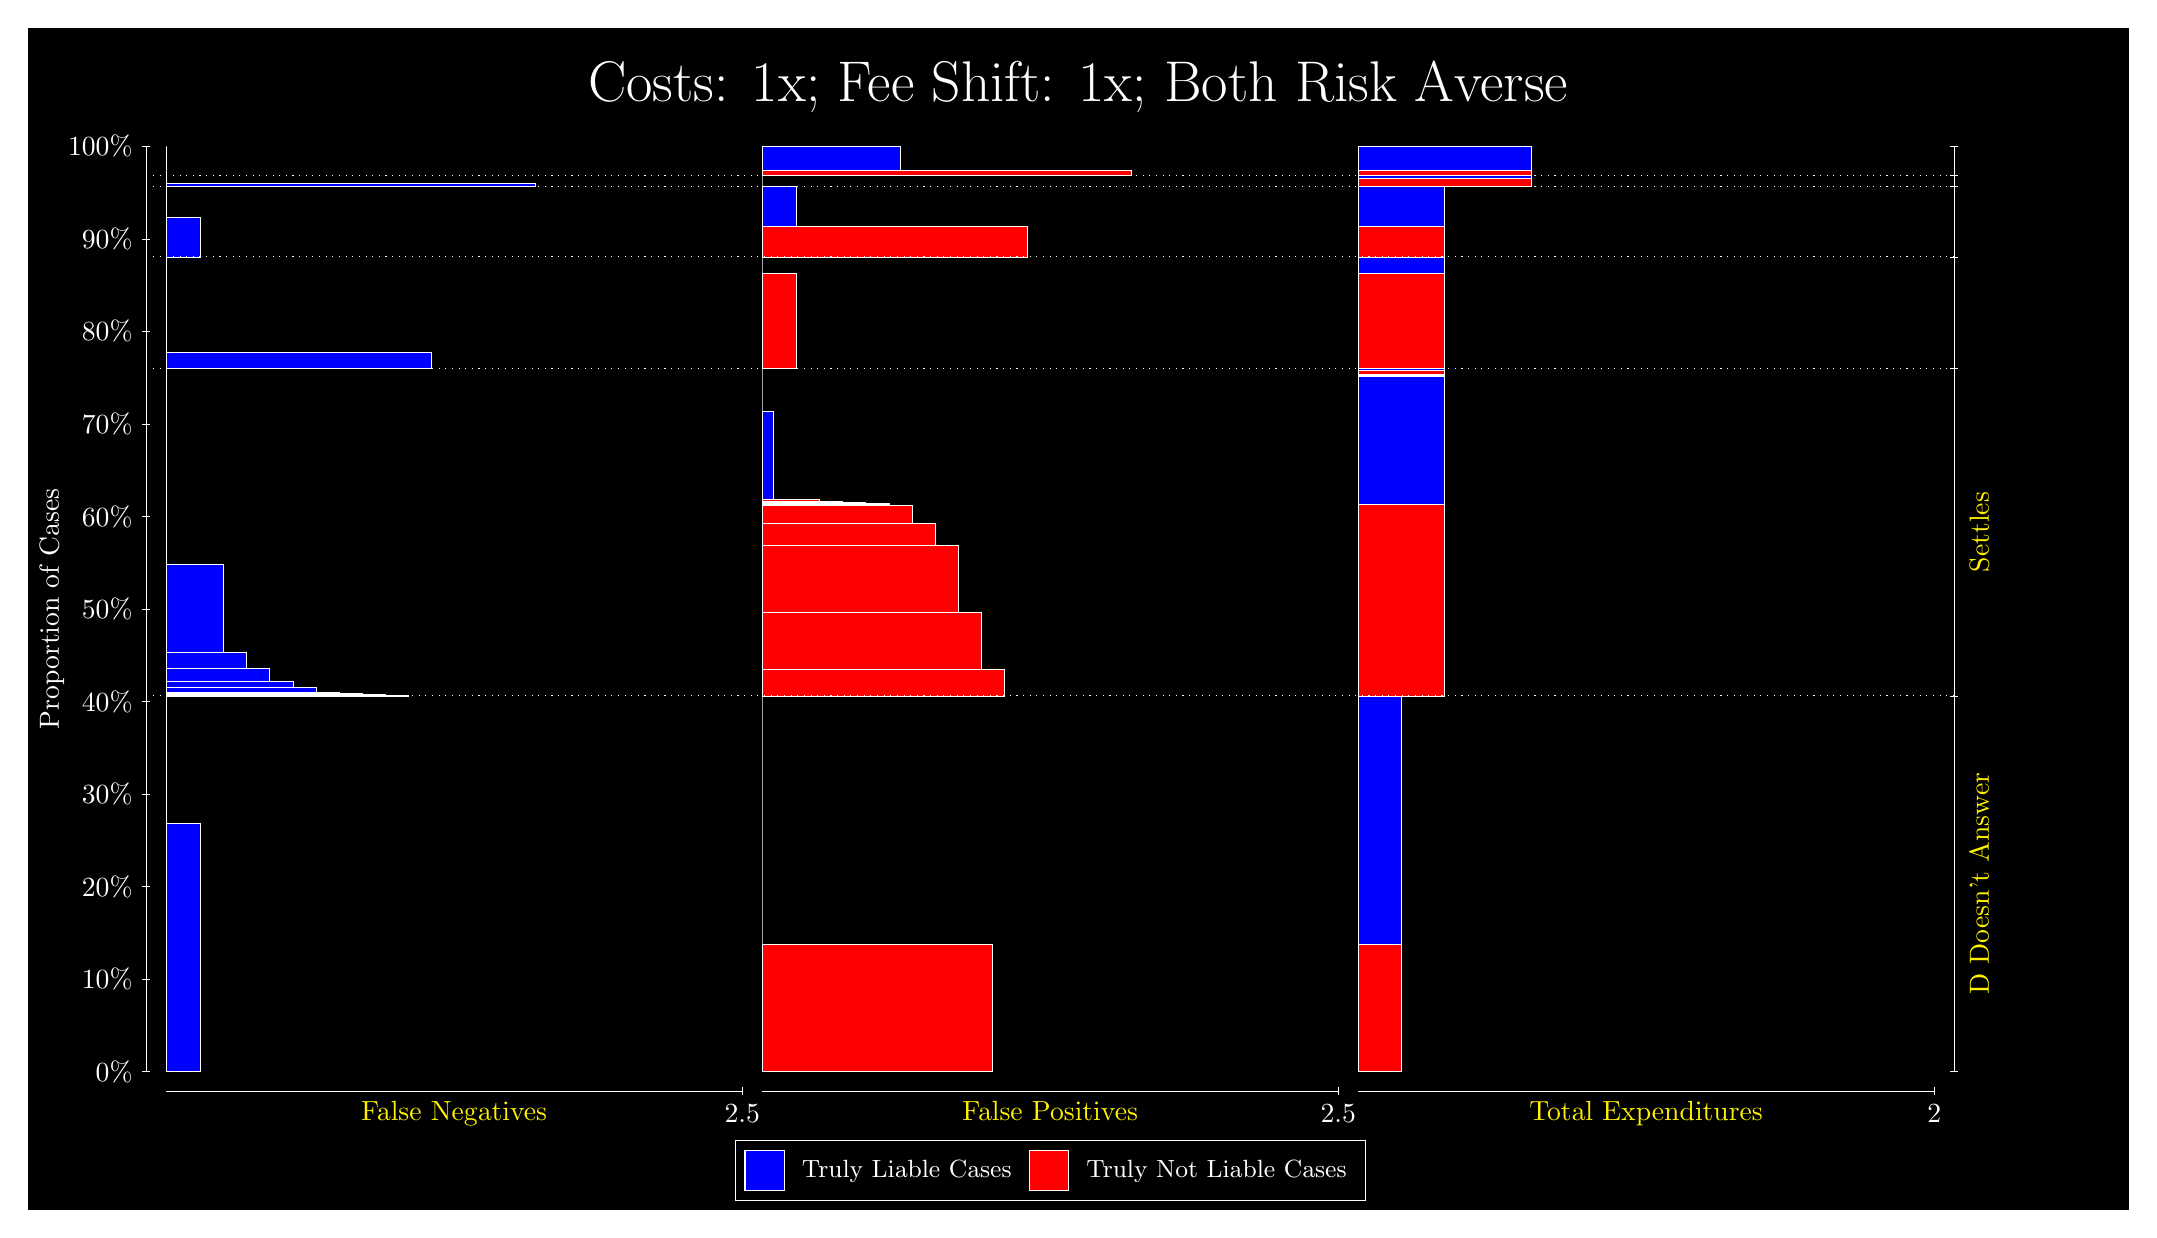
\begin{tikzpicture}
\draw[fill=black] (0,0) rectangle (26.667,15);
\draw[text=white] (0,13.5) rectangle (26.667,15) node[midway] {\huge Costs: 1x; Fee Shift: 1x; Both Risk Averse};
\draw[white, very thin] (1.5,1.75) -- (1.5,13.5);
\node[rotate=90, text=white, anchor=center] at (0.3, 7.625) {Proportion of Cases};
\draw[white, very thin] (1.45,1.75) -- (1.55,1.75);
\node[text=white, anchor=east] at (1.45, 1.75) {0\%};
\draw[white, very thin] (1.45,2.925) -- (1.55,2.925);
\node[text=white, anchor=east] at (1.45, 2.925) {10\%};
\draw[white, very thin] (1.45,4.1) -- (1.55,4.1);
\node[text=white, anchor=east] at (1.45, 4.1) {20\%};
\draw[white, very thin] (1.45,5.275) -- (1.55,5.275);
\node[text=white, anchor=east] at (1.45, 5.275) {30\%};
\draw[white, very thin] (1.45,6.45) -- (1.55,6.45);
\node[text=white, anchor=east] at (1.45, 6.45) {40\%};
\draw[white, very thin] (1.45,7.625) -- (1.55,7.625);
\node[text=white, anchor=east] at (1.45, 7.625) {50\%};
\draw[white, very thin] (1.45,8.8) -- (1.55,8.8);
\node[text=white, anchor=east] at (1.45, 8.8) {60\%};
\draw[white, very thin] (1.45,9.975) -- (1.55,9.975);
\node[text=white, anchor=east] at (1.45, 9.975) {70\%};
\draw[white, very thin] (1.45,11.15) -- (1.55,11.15);
\node[text=white, anchor=east] at (1.45, 11.15) {80\%};
\draw[white, very thin] (1.45,12.325) -- (1.55,12.325);
\node[text=white, anchor=east] at (1.45, 12.325) {90\%};
\draw[white, very thin] (1.45,13.5) -- (1.55,13.5);
\node[text=white, anchor=east] at (1.45, 13.5) {100\%};

\draw[white, very thin] (24.457,1.75) -- (24.457,13.5);
\draw[white, very thin] (24.407,1.75) -- (24.507,1.75);
\node[anchor=west] at (24.407, 1.75) {};
\draw[white, very thin] (24.407,6.5219) -- (24.507,6.5219);
\node[anchor=west] at (24.407, 6.5219) {};
\draw[white, very thin] (24.407,10.681) -- (24.507,10.681);
\node[anchor=west] at (24.407, 10.681) {};
\draw[white, very thin] (24.407,12.096) -- (24.507,12.096);
\node[anchor=west] at (24.407, 12.096) {};
\draw[white, very thin] (24.407,12.991) -- (24.507,12.991);
\node[anchor=west] at (24.407, 12.991) {};
\draw[white, very thin] (24.407,13.133) -- (24.507,13.133);
\node[anchor=west] at (24.407, 13.133) {};
\draw[white, very thin] (24.407,13.5) -- (24.507,13.5);
\node[anchor=west] at (24.407, 13.5) {};

\draw[white, very thin, fill=blue] (1.75,1.75) rectangle (2.1891,4.9035);
\draw[white, very thin, fill=red] (1.75,4.9035) rectangle (1.75,6.5219);
\draw[white, very thin, fill=blue] (1.75,6.5219) rectangle (4.8239,6.5318);
\draw[white, very thin, fill=blue] (1.75,6.5318) rectangle (4.5312,6.5387);
\draw[white, very thin, fill=blue] (1.75,6.5387) rectangle (4.2384,6.552);
\draw[white, very thin, fill=blue] (1.75,6.552) rectangle (3.9457,6.5691);
\draw[white, very thin, fill=blue] (1.75,6.5691) rectangle (3.6529,6.6354);
\draw[white, very thin, fill=blue] (1.75,6.6354) rectangle (3.3602,6.7045);
\draw[white, very thin, fill=blue] (1.75,6.7045) rectangle (3.0674,6.8697);
\draw[white, very thin, fill=blue] (1.75,6.8697) rectangle (2.7746,7.0725);
\draw[white, very thin, fill=blue] (1.75,7.0725) rectangle (2.4819,8.1907);
\draw[white, very thin, fill=red] (1.75,8.1907) rectangle (1.75,10.681);
\draw[white, very thin, fill=blue] (1.75,10.681) rectangle (5.1167,10.885);
\draw[white, very thin, fill=red] (1.75,10.885) rectangle (1.75,12.096);
\draw[white, very thin, fill=blue] (1.75,12.096) rectangle (2.1891,12.598);
\draw[white, very thin, fill=red] (1.75,12.598) rectangle (1.75,12.991);
\draw[white, very thin, fill=blue] (1.75,12.991) rectangle (6.4341,13.033);
\draw[white, very thin, fill=red] (1.75,13.033) rectangle (1.75,13.133);
\draw[white, very thin, fill=red] (1.75,13.133) rectangle (1.75,13.196);
\draw[white, very thin, fill=blue] (1.75,13.196) rectangle (1.75,13.5);
\draw[white, very thin, fill=red] (9.3189,1.75) rectangle (12.246,3.3683);
\draw[white, very thin, fill=blue] (9.3189,3.3683) rectangle (9.3189,6.5219);
\draw[white, very thin, fill=red] (9.3189,6.5219) rectangle (12.393,6.8595);
\draw[white, very thin, fill=red] (9.3189,6.8595) rectangle (12.1,7.5865);
\draw[white, very thin, fill=red] (9.3189,7.5865) rectangle (11.807,8.4286);
\draw[white, very thin, fill=red] (9.3189,8.4286) rectangle (11.515,8.7086);
\draw[white, very thin, fill=red] (9.3189,8.7086) rectangle (11.222,8.9381);
\draw[white, very thin, fill=red] (9.3189,8.9381) rectangle (10.929,8.9482);
\draw[white, very thin, fill=red] (9.3189,8.9482) rectangle (10.929,8.9636);
\draw[white, very thin, fill=red] (9.3189,8.9636) rectangle (10.636,8.9846);
\draw[white, very thin, fill=red] (9.3189,8.9846) rectangle (10.344,8.9956);
\draw[white, very thin, fill=red] (9.3189,8.9956) rectangle (10.051,9.0118);
\draw[white, very thin, fill=blue] (9.3189,9.0118) rectangle (9.4652,10.13);
\draw[white, very thin, fill=blue] (9.3189,10.13) rectangle (9.3189,10.681);
\draw[white, very thin, fill=red] (9.3189,10.681) rectangle (9.758,11.891);
\draw[white, very thin, fill=blue] (9.3189,11.891) rectangle (9.3189,12.096);
\draw[white, very thin, fill=red] (9.3189,12.096) rectangle (12.686,12.489);
\draw[white, very thin, fill=blue] (9.3189,12.489) rectangle (9.758,12.991);
\draw[white, very thin, fill=red] (9.3189,12.991) rectangle (9.3189,13.09);
\draw[white, very thin, fill=blue] (9.3189,13.09) rectangle (9.3189,13.133);
\draw[white, very thin, fill=red] (9.3189,13.133) rectangle (14.003,13.196);
\draw[white, very thin, fill=blue] (9.3189,13.196) rectangle (11.075,13.5);
\draw[white, very thin, fill=red] (16.888,1.75) rectangle (17.437,3.3683);
\draw[white, very thin, fill=blue] (16.888,3.3683) rectangle (17.437,6.5219);
\draw[white, very thin, fill=red] (16.888,6.5219) rectangle (17.986,8.9482);
\draw[white, very thin, fill=blue] (16.888,8.9482) rectangle (17.986,10.576);
\draw[white, very thin, fill=red] (16.888,10.576) rectangle (17.986,10.592);
\draw[white, very thin, fill=blue] (16.888,10.592) rectangle (17.986,10.602);
\draw[white, very thin, fill=red] (16.888,10.602) rectangle (17.986,10.65);
\draw[white, very thin, fill=blue] (16.888,10.65) rectangle (17.986,10.681);
\draw[white, very thin, fill=red] (16.888,10.681) rectangle (17.986,11.891);
\draw[white, very thin, fill=blue] (16.888,11.891) rectangle (17.986,12.096);
\draw[white, very thin, fill=red] (16.888,12.096) rectangle (17.986,12.489);
\draw[white, very thin, fill=blue] (16.888,12.489) rectangle (17.986,12.991);
\draw[white, very thin, fill=red] (16.888,12.991) rectangle (19.083,13.09);
\draw[white, very thin, fill=blue] (16.888,13.09) rectangle (19.083,13.133);
\draw[white, very thin, fill=red] (16.888,13.133) rectangle (19.083,13.196);
\draw[white, very thin, fill=blue] (16.888,13.196) rectangle (19.083,13.5);
\draw[white, dotted] (1.5,6.5219) -- (24.457,6.5219);
\draw[white, dotted] (1.5,10.681) -- (24.457,10.681);
\draw[white, dotted] (1.5,12.096) -- (24.457,12.096);
\draw[white, dotted] (1.5,12.991) -- (24.457,12.991);
\draw[white, dotted] (1.5,13.133) -- (24.457,13.133);
\draw[white, very thin] (1.75,1.5) -- (9.0689,1.5);
\node[text=yellow, anchor=north] at (5.4094, 1.5) {False Negatives};
\draw[white, very thin] (9.0689,1.45) -- (9.0689,1.55);
\node[text=white, anchor=north] at (9.0689, 1.45) {2.5};

\draw[white, very thin] (9.3189,1.5) -- (16.638,1.5);
\node[text=yellow, anchor=north] at (12.978, 1.5) {False Positives};
\draw[white, very thin] (16.638,1.45) -- (16.638,1.55);
\node[text=white, anchor=north] at (16.638, 1.45) {2.5};

\draw[white, very thin] (16.888,1.5) -- (24.207,1.5);
\node[text=yellow, anchor=north] at (20.547, 1.5) {Total Expenditures};
\draw[white, very thin] (24.207,1.45) -- (24.207,1.55);
\node[text=white, anchor=north] at (24.207, 1.45) {2};

\node[text=yellow, centered, rotate=90] at (24.777, 4.1359) {D Doesn't Answer};
\node[text=yellow, centered, rotate=90] at (24.777, 8.6013) {Settles};





\draw (12.978300999999998,1.5) node[draw=none] (baseCoordinate) {};
\begin{scope}[align=center]
        \matrix[scale=0.5, draw=white, below=0.5cm of baseCoordinate, nodes={draw}, column sep=0.1cm]{
            \node[rectangle, draw, minimum width=0.5cm, minimum height=0.5cm, fill=blue] {}; &
            \node[draw=none, font=\small, text=white] (B) {Truly Liable Cases}; &
            \node[rectangle, draw, minimum width=0.5cm, minimum height=0.5cm, fill=red] {}; &
            \node[draw=none, font=\small, text=white] (B) {Truly Not Liable Cases}; \\
            };
\end{scope}

\end{tikzpicture}
\end{document}